\documentclass[10pt,a4paper]{article}
\usepackage[utf8]{inputenc}
\usepackage[english]{babel}
\usepackage[T1]{fontenc}
\usepackage{amsmath}
\usepackage{amsfonts}
\usepackage{amssymb}
\usepackage{lmodern}
\usepackage{fancyvrb}

%\usepackage{dot2texi}
\usepackage{tikz}
\usetikzlibrary{shapes,arrows}

\newcommand{\version}{\IfFileExists{../../version.txt}
{\input{../../version.txt}}
{\input{../../../version.txt}}
}

\newcommand{\command}[1]{%
\indent \fcolorbox{black}{white}{%
   \begin{minipage}{\dimexpr\textwidth-\parindent\relax}%
      #1
   \end{minipage}%
}
}

\newsavebox{\FVerbBox}
\newenvironment{sample}
{\par \vspace{0.2cm} \begin{lrbox}{\FVerbBox}
\begin{minipage}{\dimexpr\textwidth-\parindent\relax}}
{\end{minipage}
\end{lrbox}
\fcolorbox{black}{lightgray}{\usebox{\FVerbBox}}
\vspace{0.2cm}}

\newenvironment{sampletitle}
{\vspace{0.2cm} \noindent\textbf{Example} :
\begin{sample}}
{\end{sample}}

\newcommand{\samplecomment}[1]{%

\textit{#1}
}

\newcommand{\seealso}[1]{\vspace{0.2cm} \noindent\textbf{See also} :\par #1}

% tikz
\usetikzlibrary{calc}
\usetikzlibrary{arrows}
\usetikzlibrary{shadows}

\tikzset{block/.style={draw, text centered, fill=gray!10,drop shadow}}
\tikzset{connect/.style={draw, line width=1 pt}}

\author{Sebastien CAUX}
\title{GPStudio Tutorial \version : \\ 2. How to create and use a simple node project in command line mode?}

\begin{document}
\maketitle
\section{Introduction}
This tutorial is done to show how GPStudio is simple to use when you are using only IP in library on a supported board. For this example, we use the famous Dreamcam platform, the firt platform supported by GPStudio.\\

In this tutorial, we create a project for a specific platform and configure the platform. After that, we add some process in the project, setting up and connect process each other.

Finally, we configure the smart camera with the compiled project and check results of processing on viewer interface.

\section{Driving the flow from image sensor to USB}
\subsection{Create the project and configure platform}
First of all, you need to create the project in an empty directory :

\textbf{setenv}\\

\sample{
> mkdir tuto1\\
> cd tuto1\\
> \textbf{gpnode} \textbf{newproject} -n tuto1
}

After that, you should have a file named \emph{tuto1.node} in the current directory. This file is the project file and contain the definition of the node. Please notify that you can have only one project file per directory and gpnode always works on the project in the current directory. The directory name could be different that the project name, but you should not modify the name of the project file.\\

The next thing to do is to specify the platform that you want to use for this project. You can do it with :

\sample{
> \textbf{gpnode} \textbf{setboard} -n dreamcam\_c3
}

`dreamcam\_c3' corresponds to a DreamCam platform with Cyclone III FPGA. The board support package for the `dreamcam\_c3' camera is located at :

\emph{<gps-root>/support/board/dreamcam\_c3/dreamcam\_c3.dev}

DreamCam is now set as target platform. You can check that with the command showboard :

\sample{
> \textbf{gpnode} \textbf{showboard}\\
dreamcam\_c3}

\subsection{Add IO support that you need}
Until now, we only specify the Dreamcam as platform, but it is a modular one, you can use different types of image sensor and communication. It require to define witch one we want to use by adding the support of theses peripherals. \\

command to know available ios

For image sensor, you have two possibilities, mt9 from Aptina or e2v. For this example, we choose mt9 :

\sample{
> \textbf{gpnode} \textbf{addio} -n mt9
}

By adding mt9 IO, gpnode fetch the name of the driver to use with this IO and copy the driver files implementation. Like that, it allows you to use it to capture pictures from this sensor.\\

Now, for enable a communication, you have the choice between Ethernet or USB. Choose USB support :

\sample{
> \textbf{gpnode} \textbf{addio} -n usb
}

You can view the list of ios support with the command showio :

\sample{
> \textbf{gpnode} \textbf{showio}\\
ios :\\
 + mt9 [mt9]\\
 + usb [usb\_cypress\_CY7C68014A]
}

\subsection{Connect block flow}

\begin{figure}[h!]
\centering
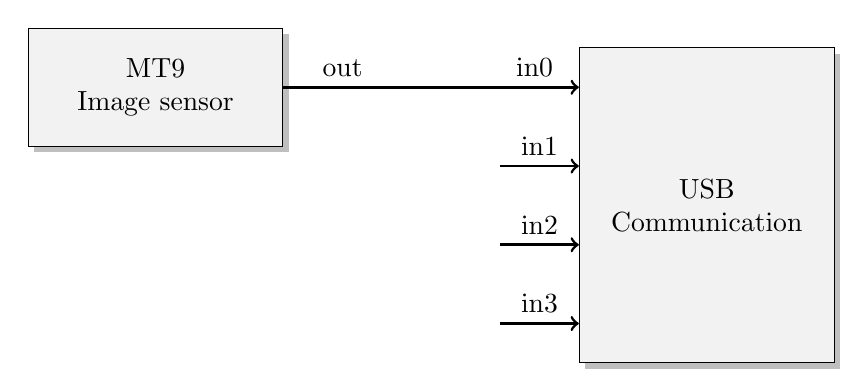
\begin{tikzpicture}[node distance=8cm]

\tikzset{blocstyle/.style={block,rectangle,minimum height=1.5cm,text width=3cm}};

% blocks
\node[blocstyle] (bloc1) {MT9\\Image sensor};
\node[blocstyle,minimum height=4cm] (bloc2) at (7,-1.5) {USB\\Communication};

% Flow to
%\path[connect,->] ([yshift=0.5cm]bloc1.east) -- node[above]{flow1\_data} node{/} ([yshift=0.5cm]bloc2.west);
%\path[connect,->] (bloc1.east) -- node[above]{flow1\_dv} (bloc2.west);
%\path[connect,->] ([yshift=-0.5cm]bloc1.east) -- node[above]{flow1\_fv} ([yshift=-0.5cm]bloc2.west);
\path[connect,->] (bloc1.east) -- node[above,pos=0.2]{out} node[above,pos=0.85]{in0} ([yshift=1.5cm]bloc2.west);
\path[connect,<-] ([yshift=0.5cm]bloc2.west) -- node[above]{in1} ++(-1,0);
\path[connect,<-] ([yshift=-0.5cm]bloc2.west) -- node[above]{in2} ++(-1,0);
\path[connect,<-] ([yshift=-1.5cm]bloc2.west) -- node[above]{in3} ++(-1,0);

\end{tikzpicture}
\caption{Details on flow connexion}
\end{figure}


\sample{
> \textbf{gpnode} \textbf{connect} -f mt9.out -t usb.in0
}

\sample{
> \textbf{gpnode} \textbf{showconnects}\\
connects :\\
  + mt9.out -> usb.in0 (msb)}

\section{Adding a process from GPStudio library}
\subsection{Add process that you need}


\sample{> \textbf{gpnode} \textbf{addprocess} -n process1 -d gradienthw}

\sample{
> \textbf{gpnode} \textbf{showprocess}\\process :\\ + process1 [gradienthw]}


\end{document}
